\begin{figure}

\centering



\tikzset{every picture/.style={line width=0.75pt}} %set default line width to 0.75pt        

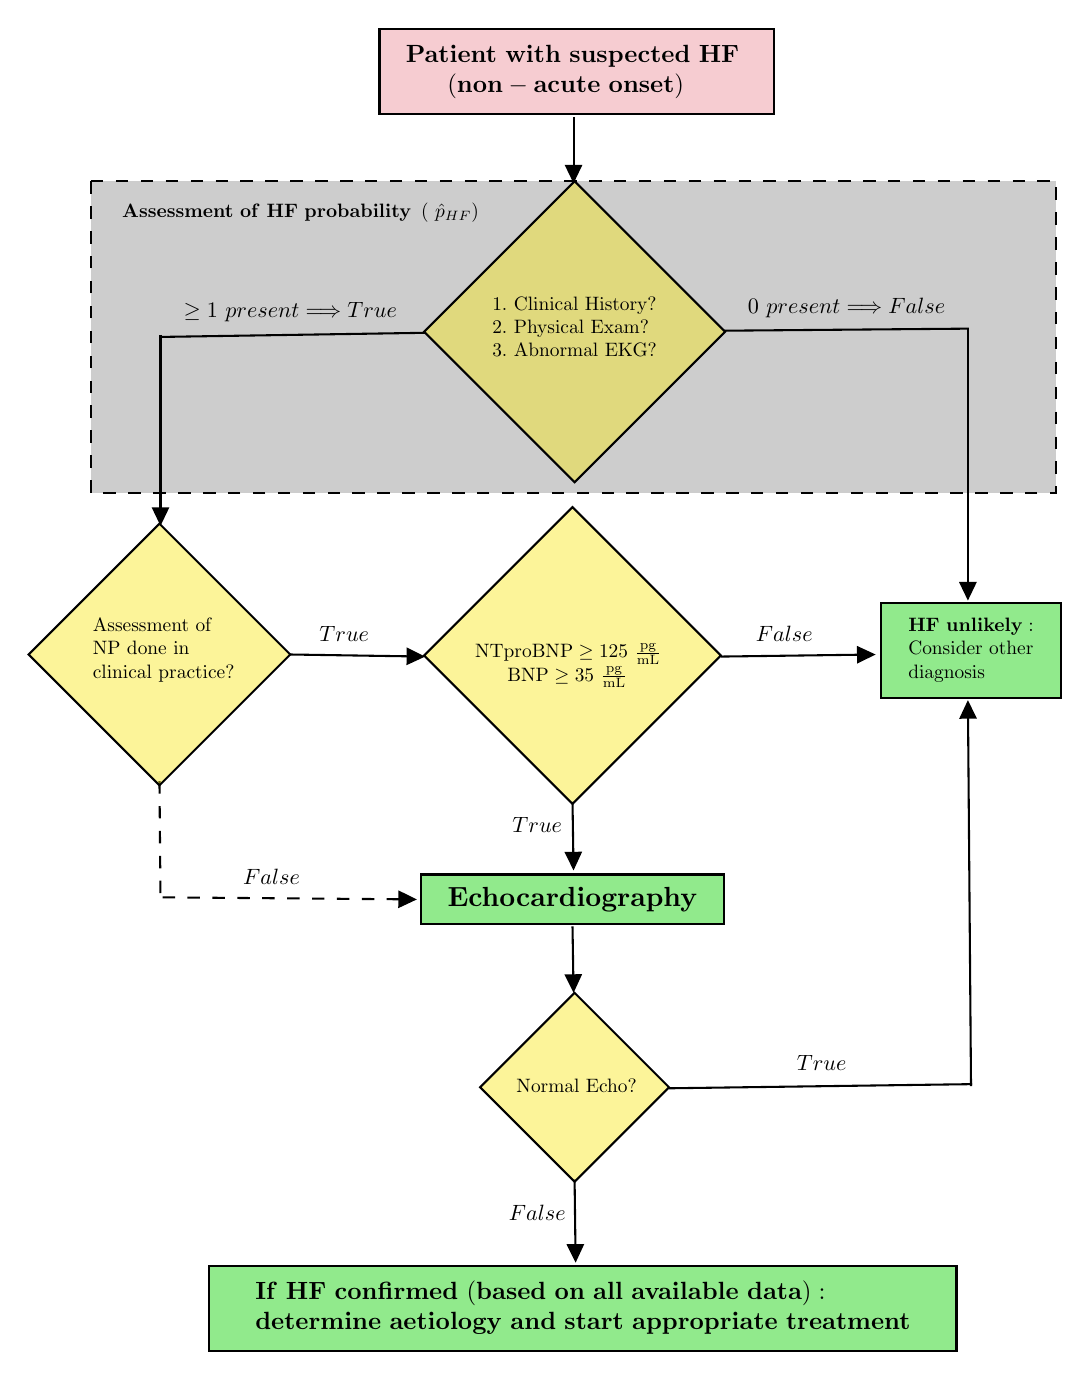
\begin{tikzpicture}[x=0.75pt,y=0.75pt,yscale=-1,xscale=1]
%uncomment if require: \path (0,652); %set diagram left start at 0, and has height of 652

%Shape: Rectangle [id:dp05338957976791869] 
\draw  [fill={rgb, 255:red, 155; green, 155; blue, 155 }  ,fill opacity=0.5 ][dash pattern={on 4.5pt off 4.5pt}] (35,80) -- (500,80) -- (500,230) -- (35,230) -- cycle ;
%Straight Lines [id:da055858825280932] 
\draw    (267.5,49) -- (267.5,79) ;
\draw [shift={(267.5,81)}, rotate = 270] [fill={rgb, 255:red, 0; green, 0; blue, 0 }  ][line width=0.75]  [draw opacity=0] (8.93,-4.29) -- (0,0) -- (8.93,4.29) -- cycle    ;

%Straight Lines [id:da4365110914453669] 
\draw    (68.5,155) -- (196.5,153) ;


%Straight Lines [id:da3272244813405638] 
\draw    (68.5,154) -- (68.5,244) ;
\draw [shift={(68.5,246)}, rotate = 270] [fill={rgb, 255:red, 0; green, 0; blue, 0 }  ][line width=0.75]  [draw opacity=0] (8.93,-4.29) -- (0,0) -- (8.93,4.29) -- cycle    ;

%Straight Lines [id:da17400033500022816] 
\draw    (457.5,151) -- (457.5,280) ;
\draw [shift={(457.5,282)}, rotate = 270] [fill={rgb, 255:red, 0; green, 0; blue, 0 }  ][line width=0.75]  [draw opacity=0] (8.93,-4.29) -- (0,0) -- (8.93,4.29) -- cycle    ;

%Straight Lines [id:da3278613507085377] 
\draw    (131,308) -- (194,308.97) ;
\draw [shift={(196,309)}, rotate = 180.88] [fill={rgb, 255:red, 0; green, 0; blue, 0 }  ][line width=0.75]  [draw opacity=0] (8.93,-4.29) -- (0,0) -- (8.93,4.29) -- cycle    ;

%Shape: Square [id:dp3364304080096274] 
\draw  [fill={rgb, 255:red, 248; green, 231; blue, 28 }  ,fill opacity=0.45 ] (268,80) -- (340.5,152.5) -- (268,225) -- (195.5,152.5) -- cycle ;
%Straight Lines [id:da1685251091101021] 
\draw    (340,152) -- (458,151) ;


%Straight Lines [id:da2968793712930289] 
\draw    (338.5,309) -- (411,308.03) ;
\draw [shift={(413,308)}, rotate = 539.23] [fill={rgb, 255:red, 0; green, 0; blue, 0 }  ][line width=0.75]  [draw opacity=0] (8.93,-4.29) -- (0,0) -- (8.93,4.29) -- cycle    ;

%Straight Lines [id:da5449359734131121] 
\draw  [dash pattern={on 4.5pt off 4.5pt}]  (69.5,425) -- (190,425.98) ;
\draw [shift={(192,426)}, rotate = 180.47] [fill={rgb, 255:red, 0; green, 0; blue, 0 }  ][line width=0.75]  [draw opacity=0] (8.93,-4.29) -- (0,0) -- (8.93,4.29) -- cycle    ;

%Straight Lines [id:da5016779396235063] 
\draw  [dash pattern={on 4.5pt off 4.5pt}]  (68,369) -- (68.5,426) ;


%Straight Lines [id:da7236757292406453] 
\draw    (267,439) -- (267.47,469) ;
\draw [shift={(267.5,471)}, rotate = 269.1] [fill={rgb, 255:red, 0; green, 0; blue, 0 }  ][line width=0.75]  [draw opacity=0] (8.93,-4.29) -- (0,0) -- (8.93,4.29) -- cycle    ;

%Straight Lines [id:da760594202182669] 
\draw    (313.5,517) -- (459.5,515) ;


%Straight Lines [id:da3750532871622436] 
\draw    (459,516) -- (457.52,332) ;
\draw [shift={(457.5,330)}, rotate = 449.54] [fill={rgb, 255:red, 0; green, 0; blue, 0 }  ][line width=0.75]  [draw opacity=0] (8.93,-4.29) -- (0,0) -- (8.93,4.29) -- cycle    ;

%Shape: Square [id:dp7874754730652669] 
\draw  [fill={rgb, 255:red, 248; green, 231; blue, 28 }  ,fill opacity=0.45 ] (267,237) -- (338.5,308.5) -- (267,380) -- (195.5,308.5) -- cycle ;
%Shape: Square [id:dp19176781264401277] 
\draw  [fill={rgb, 255:red, 248; green, 231; blue, 28 }  ,fill opacity=0.45 ] (68,245) -- (131,308) -- (68,371) -- (5,308) -- cycle ;
%Shape: Square [id:dp8240263825354897] 
\draw  [fill={rgb, 255:red, 248; green, 231; blue, 28 }  ,fill opacity=0.45 ] (268,471) -- (313.5,516.5) -- (268,562) -- (222.5,516.5) -- cycle ;
%Straight Lines [id:da9916785343630015] 
\draw    (267,379) -- (267.47,410) ;
\draw [shift={(267.5,412)}, rotate = 269.13] [fill={rgb, 255:red, 0; green, 0; blue, 0 }  ][line width=0.75]  [draw opacity=0] (8.93,-4.29) -- (0,0) -- (8.93,4.29) -- cycle    ;

%Straight Lines [id:da8876972127593497] 
\draw    (268,561) -- (268.48,599) ;
\draw [shift={(268.5,601)}, rotate = 269.28] [fill={rgb, 255:red, 0; green, 0; blue, 0 }  ][line width=0.75]  [draw opacity=0] (8.93,-4.29) -- (0,0) -- (8.93,4.29) -- cycle    ;


% Text Node
\draw  [fill={rgb, 255:red, 139; green, 233; blue, 134 }  ,fill opacity=0.95 ]  (194,414) -- (340,414) -- (340,438) -- (194,438) -- cycle  ;
\draw (267,426) node [scale=1]  {$\mathbf{Echocardiography}$};
% Text Node
\draw  [fill={rgb, 255:red, 139; green, 233; blue, 134 }  ,fill opacity=0.95 ]  (415.5,283) -- (502.5,283) -- (502.5,329) -- (415.5,329) -- cycle  ;
\draw (459,306) node [scale=0.7]  {$ \begin{array}{l}
\mathbf{HF\ unlikely:}\\
\mathrm{Consider\ other}\\
\mathrm{diagnosis}
\end{array}$};
% Text Node
\draw (157,298) node [scale=0.8]  {$True$};
% Text Node
\draw (369,298) node [scale=0.8]  {$False$};
% Text Node
\draw (250,390) node [scale=0.8]  {$True$};
% Text Node
\draw (122,415) node [scale=0.8]  {$False$};
% Text Node
\draw (136,95) node [scale=0.7]  {$\mathbf{Assessment\ of\ HF\ probability} \ \left( \ \hat{p}_{HF}\right)$};
% Text Node
\draw (387,505) node [scale=0.8]  {$True$};
% Text Node
\draw (250,577) node [scale=0.8]  {$False$};
% Text Node
\draw (268,151) node [scale=0.7]  {$ \begin{array}{l}
\mathrm{1.\ Clinical\ History?}\\
\mathrm{2.\ Physical\ Exam?}\\
\mathrm{3.\ Abnormal\ EKG?}
\end{array}$};
% Text Node
\draw (131,143) node [scale=0.8]  {$\geq 1\ present\Longrightarrow True$};
% Text Node
\draw (399,141) node [scale=0.8]  {$0\ present\Longrightarrow False$};
% Text Node
\draw (70,306) node [scale=0.7]  {$ \begin{array}{l}
\mathrm{Assessment\ of\ }\\
\mathrm{NP\ done\ in\ }\\
\mathrm{clinical\ practice?}
\end{array}$};
% Text Node
\draw (265,313) node [scale=0.7]  {$ \begin{array}{l}
\mathrm{NTproBNP\geq 125\ \frac{pg}{mL}}\\
\mathrm{\ \ \ \ \ BNP\geq 35\ \frac{pg}{mL}}
\end{array}$};
% Text Node
\draw  [fill={rgb, 255:red, 139; green, 233; blue, 134 }  ,fill opacity=0.95 ]  (92,602.5) -- (452,602.5) -- (452,643.5) -- (92,643.5) -- cycle  ;
\draw (272,623) node [scale=0.9]  {$ \begin{array}{l}
\mathbf{If\ HF\ confirmed\ ( based\ on\ all\ available\ data) :}\\
\mathbf{determine\ aetiology\ and\ start\ appropriate\ treatment}
\end{array}$};
% Text Node
\draw (269,516) node [scale=0.7]  {$\mathrm{Normal\ Echo?}$};
% Text Node
\draw  [fill={rgb, 255:red, 208; green, 2; blue, 27 }  ,fill opacity=0.2 ]  (174,6.5) -- (364,6.5) -- (364,47.5) -- (174,47.5) -- cycle  ;
\draw (269,27) node [scale=0.9]  {$ \begin{array}{l}
\mathbf{Patient\ with\ suspected\ HF\ }\\
\mathbf{\ \ \ \ \ ( non-acute\ onset)}
\end{array}$};


\end{tikzpicture}

\caption[ESC diagnostic algorithm of heart failure]{\textit{ESC diagnostic algorithm for the diagnosis of heart failure of non-acute onset \cite[page.~2141]{ponikowski2016}.}}
\label{fig:esc_algo_hf}
\normalsize
\end{figure}